% 
% Septiembre 2020
% Author: Mathieu Kessler
% Universidad Politécnica de Cartagena
% https://personas.upct.es/perfil/mathieu.kessler
% 
% 
\documentclass[handout,9pt]{beamer}
\definecolor{links}{HTML}{2A1B81}
\hypersetup{colorlinks,linkcolor=,urlcolor=links}
 \usepackage[spanish]{babel}
\usepackage{colortbl}
\usepackage{graphicx}
\usepackage{amsmath,amssymb}
\usepackage{comma}
\usepackage{fancybox,color}
\usepackage[utf8]{inputenc}
\graphicspath{{../../transparencias/figures/}}
\setbeamertemplate{navigation symbols}{}
% -----------------------------------------------------------------------------
% To include multple images sequentially
% https://codeyarns.com/2010/02/09/how-to-do-image-animation-in-beamer/
% ------------------------------------------------------------------------------
 \usepackage{xmpmulti}
%------------------------------------------------------------------------------
\usepackage{xcolor}
\definecolor{mycodecolor}{rgb}{0.65,0.25,0.1}
\newcommand{\inlinecode}[1]{{\tt \textcolor{mycodecolor}{#1}}}
\usepackage{pythontex}
%--------------------
\usepackage{beamerthemeshadow}
\usepackage{xmpmulti}
\usepackage{mathtools}
\DeclarePairedDelimiter\abs{\lvert}{\rvert}%
\usepackage{tabularx}
\renewcommand\tabularxcolumn[1]{b{#1}}
\newcommand{\field}[1]{\mathbb{#1}}
\newcommand{\E}{\field{E}}
\newcommand{\R}{\field{R}}
\newcommand{\N}{\field{N}}
\newcommand{\Z}{\field{Z}}
\newcommand{\Q}{\field{Q}}
\newcommand{\EE}{\field{E}}
\newcommand{\FF}{\field{F}}
\newcommand{\GG}{\field{G}}
\renewcommand{\L}{\field{L}}
\renewcommand{\P}{\field{P}}
\newcommand{\LL}{{\mathfrak L}}

% define el folder donde del workspace, para cambiar inglés, ids,
% etc..
\newcommand{\workspacefolder}{stat\_labs }


\begin{document}
\title{Ejercicios de acompañamiento a ``Python: una introducción
  básica'' y ``Más sobre listas y diccionarios'' }

\author[Mathieu Kessler]{Mathieu Kessler}
\institute[]{Departamento de Matemática Aplicada y Estadística \\ Universidad Politécnica de Cartagena}
\date{@kessler\_mathieu}{}%{\href{https://code.visualstudio.com}{https://code.visualstudio.com}}
\titlegraphic{
\includegraphics[width=3cm]{python_logo}}

\begin{frame}
  \titlepage
\end{frame}

\begin{frame}[fragile]
  \frametitle{Ejercicios}
  \begin{description}
    \item[Ejercicio 1] Escribe un programa en un fichero {\tt ejercicios\_introduccion.py} que
      pide un entero \pyv{n} al usuario y imprime en consola la suma
      de los primeros  \pyv{n} términos de la secuencia $4$, $-4/3$, $4/5$, $-4/7
      \ldots$, i.e. la secuencia
      $$ 4\times \frac{(-1)^{i}}{2\cdot i + 1},\ i = 0, 1, 2, \ldots$$
      \begin{itemize}
      \item \textit{Indicación 1: El operador de potencia en Python es
          \pyv{**}.}
      \item \textit{Indicación 2: Que no se os olvide de usar
          \pyv{int(n)} para transformar el input a un entero.}
      \end{itemize}
      Ejecutad vuestro programa con valores de $n$ grandes.
    \item[Ejercicio 2] Añadid a vuestro programa anterior
            las instrucciones para devolver la tabla de multiplicación
      de $n$, que ha introducido el usuario.

    \end{description}  
  \end{frame}

\begin{frame}
  \frametitle{Ejercicios}
  \begin{description}
        \item[Ejercicio 3] Añadid a vuestro programa las instrucciones
          para imprimir el siguiente patrón, pudiendo especificar el
          número de filas:
      \begin{center}
        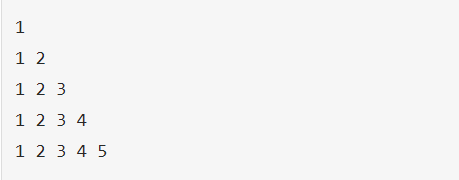
\includegraphics[width=5cm]{for_exercises_01}
      \end{center}
      
  \item[Ejercicio 4] Completad vuestro programa en {\tt ejercicios\_introduccion.py}
    con las  instrucciones para comprobar si $n$ introducido por el usuario es un
    número primo.
  \item[Ejercicio 5] Añadid a vuestro programa en {\tt ejercicios\_introduccion.py}
    la definición de una función que tenga el entero \pyv{n} como
    argumento y que devuelva \pyv{True} si \pyv{n} es un número primo
    y  \pyv{False} en otro caso.
  \item[Ejercicio 6] Añadid al programa las instrucciones que permitan imprimir
    todos los números primos inferiores a \pyv{n}, introducido por el usuario.
  \end{description}  
\end{frame}


  \begin{frame}[fragile]
  \frametitle{Comprehensiones de listas o diccionarios}
Consideramos el diccionario de personas:
\begin{pyconsole}
personas = {
   'Pedro': 28,
   'María': 21,
   'Marta': 22
}
\end{pyconsole}
\begin{block}{Ejercicio 7 (reto):}
 Si consigo del INE la esperanza de vida adicional en años para cada
 de sus edades:
 \begin{pyverbatim}
esperanza_adicional = {
     28: 53.4
     21: 65.6
     22: 64,5
}
 \end{pyverbatim}
Podríais construir un diccionario con la esperanza de vida de  Pedro, María y
Marta?
\end{block}
\end{frame}
  
\end{document}
